% Text-free, transparent-background base of the six-process PEM-cell graphic.
\documentclass[tikz,border=0pt]{standalone}
\usepackage{tikz}
\usetikzlibrary{arrows.meta}

\definecolor{electric}{HTML}{4F83C6}
\definecolor{reaction}{HTML}{D88724}
\definecolor{gas}{HTML}{5DB5C9}
\definecolor{water}{HTML}{527FB5}
\definecolor{thermal}{HTML}{D76C57}
\definecolor{voltage}{HTML}{92AA49}

\begin{document}
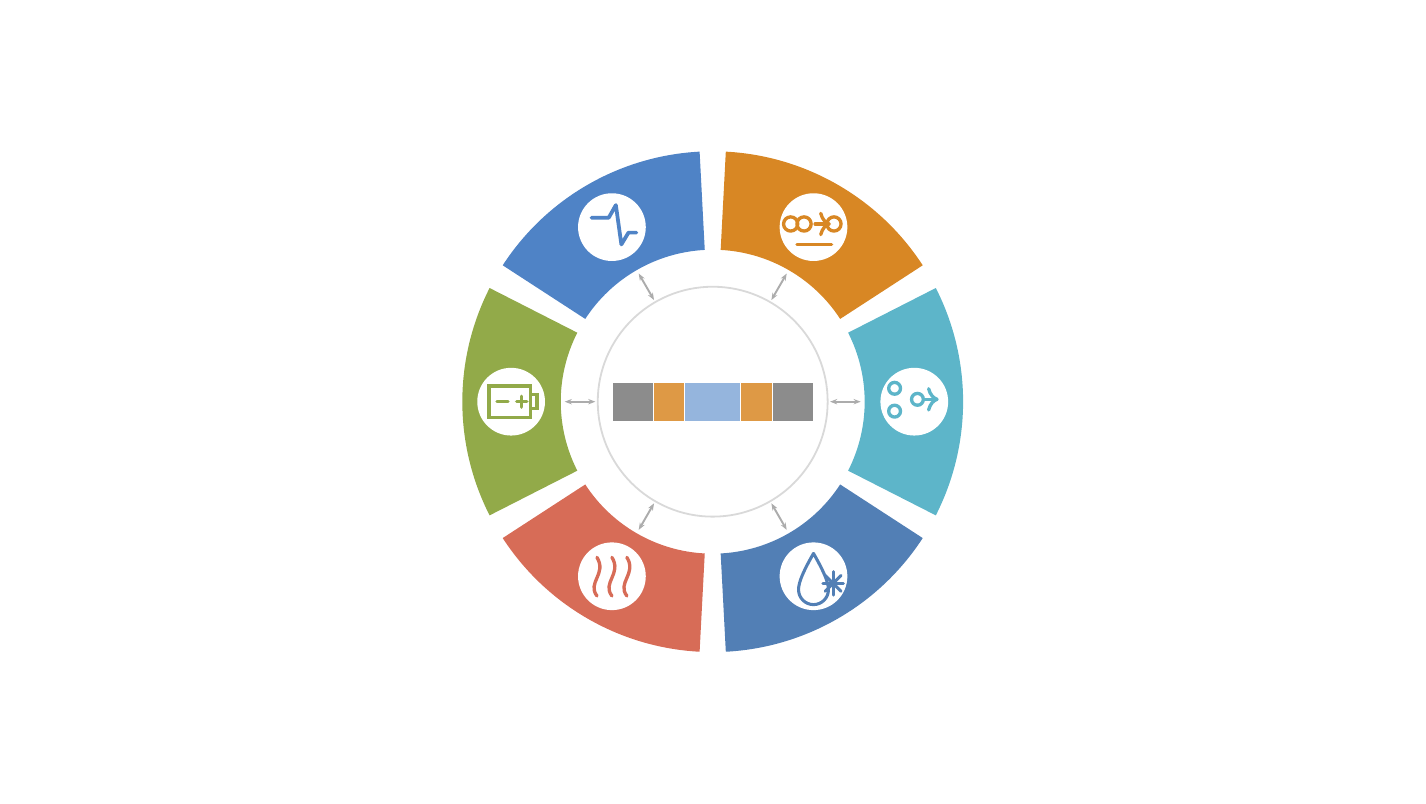
\begin{tikzpicture}[x=1cm,y=1cm]
  \path[use as bounding box] (-8.7,-4.75) rectangle (8.7,4.75);

  \foreach \mid/\col in {120/electric,60/reaction,0/gas,-60/water,-120/thermal,180/voltage}{
    \pgfmathsetmacro{\aa}{\mid-27}
    \pgfmathsetmacro{\bb}{\mid+27}
    \fill[\col] (\aa:1.93)
      arc[start angle=\aa,end angle=\bb,radius=1.93]
      -- (\bb:3.18)
      arc[start angle=\bb,end angle=\aa,radius=3.18] -- cycle;
    \fill[white] (\mid:2.56) circle[radius=0.43];
    \draw[gray!65,line width=0.7pt,
      {Stealth[length=2.6pt]}-{Stealth[length=2.6pt]}]
      (\mid:1.49) -- (\mid:1.88);
  }

  \fill[white] (0,0) circle[radius=1.46];
  \draw[gray!30,line width=0.65pt] (0,0) circle[radius=1.46];

  % Five physical layers: aGDL, aCL, PEM, cCL, cGDL.
  \fill[black!45] (-1.27,-0.24) rectangle (-0.76,0.24);
  \fill[reaction!85] (-0.75,-0.24) rectangle (-0.36,0.24);
  \fill[electric!60] (-0.35,-0.24) rectangle (0.35,0.24);
  \fill[reaction!85] (0.36,-0.24) rectangle (0.75,0.24);
  \fill[black!45] (0.76,-0.24) rectangle (1.27,0.24);

  % Current-transfer pulse.
  \begin{scope}[shift={(120:2.56)},draw=electric,line width=1.35pt,line cap=round,line join=round]
    \draw (-0.26,0.12) -- (-0.04,0.12) -- (0.05,0.28) -- (0.12,-0.22)
      -- (0.21,-0.07) -- (0.31,-0.07);
  \end{scope}
  % Electrochemical reaction.
  \begin{scope}[shift={(60:2.56)},draw=reaction,line width=1.2pt,line cap=round]
    \draw (-0.29,0.04) circle[radius=0.09];
    \draw (-0.12,0.04) circle[radius=0.09];
    \draw[->] (0.02,0.04) -- (0.22,0.04);
    \draw (0.26,0.04) circle[radius=0.09];
    \draw (-0.21,-0.22) -- (0.23,-0.22);
  \end{scope}
  % Gas diffusion.
  \begin{scope}[shift={(0:2.56)},draw=gas,line width=1.2pt,line cap=round]
    \draw (-0.25,0.17) circle[radius=0.075];
    \draw (-0.25,-0.12) circle[radius=0.075];
    \draw (0.04,0.03) circle[radius=0.075];
    \draw[->] (0.12,0.03) -- (0.31,0.03);
  \end{scope}
  % Liquid water and ice.
  \begin{scope}[shift={(-60:2.56)},draw=water,line width=1.1pt,line cap=round]
    \draw (0,0.29) .. controls (-0.12,0.08) and (-0.19,-0.07) .. (-0.19,-0.17)
      arc[start angle=180,end angle=360,radius=0.19]
      .. controls (0.19,-0.07) and (0.12,0.08) .. (0,0.29);
    \draw (0.25,0.06) -- (0.25,-0.24);
    \draw (0.12,-0.09) -- (0.38,-0.09);
    \draw (0.15,0.01) -- (0.35,-0.19);
    \draw (0.35,0.01) -- (0.15,-0.19);
  \end{scope}
  % Heat waves.
  \begin{scope}[shift={(-120:2.56)},draw=thermal,line width=1.2pt,line cap=round]
    \foreach \xx in {-0.19,0,0.19}{
      \draw (\xx,-0.25) .. controls (\xx-0.13,-0.08) and (\xx+0.13,0.03) .. (\xx,0.24);
    }
  \end{scope}
  % Battery and polarity marks are vector strokes, not text.
  \begin{scope}[shift={(180:2.56)},draw=voltage,line width=1.2pt,line cap=round]
    \draw (-0.28,-0.2) rectangle (0.25,0.2);
    \draw (0.25,-0.09) -- (0.33,-0.09) -- (0.33,0.09) -- (0.25,0.09);
    \draw (-0.18,0) -- (-0.04,0);
    \draw (0.07,0) -- (0.2,0);
    \draw (0.135,-0.07) -- (0.135,0.07);
  \end{scope}
\end{tikzpicture}
\end{document}
